\begin{figure}
    \centering
    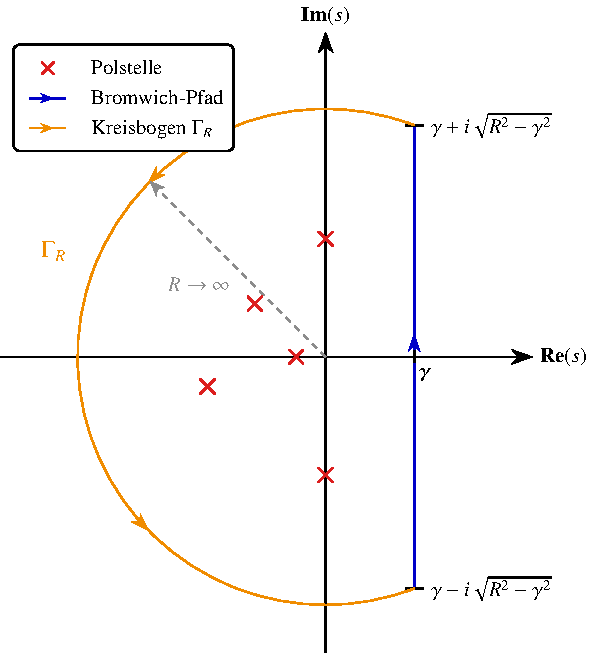
\includegraphics{papers/laplace/images/d_kontur.pdf}
    \caption{Die geschlossene D-Kontur:
    Der vertikale Bromwich-Pfad bildet die Sehne eines im Ursprung
    zentrierten Kreises, dessen grosser Bogen $\Gamma_R$ die Kurve nach
    links schliesst und dabei im Streifen $0 < \text{Re}(s) < \gamma$
    leicht in die rechte Halbebene hineinragt.
    Für $R \to \infty$ umschliesst die Kurve alle Singularitäten von
    $F(s)$, während der Beitrag des Bogens nach dem Lemma von Jordan
    verschwindet.}
    \label{laplace:fig:d_kontur}
\end{figure}
